\documentclass{article}\usepackage[]{graphicx}\usepackage[]{color}
% maxwidth is the original width if it is less than linewidth
% otherwise use linewidth (to make sure the graphics do not exceed the margin)
\makeatletter
\def\maxwidth{ %
  \ifdim\Gin@nat@width>\linewidth
    \linewidth
  \else
    \Gin@nat@width
  \fi
}
\makeatother

\definecolor{fgcolor}{rgb}{0.345, 0.345, 0.345}
\newcommand{\hlnum}[1]{\textcolor[rgb]{0.686,0.059,0.569}{#1}}%
\newcommand{\hlstr}[1]{\textcolor[rgb]{0.192,0.494,0.8}{#1}}%
\newcommand{\hlcom}[1]{\textcolor[rgb]{0.678,0.584,0.686}{\textit{#1}}}%
\newcommand{\hlopt}[1]{\textcolor[rgb]{0,0,0}{#1}}%
\newcommand{\hlstd}[1]{\textcolor[rgb]{0.345,0.345,0.345}{#1}}%
\newcommand{\hlkwa}[1]{\textcolor[rgb]{0.161,0.373,0.58}{\textbf{#1}}}%
\newcommand{\hlkwb}[1]{\textcolor[rgb]{0.69,0.353,0.396}{#1}}%
\newcommand{\hlkwc}[1]{\textcolor[rgb]{0.333,0.667,0.333}{#1}}%
\newcommand{\hlkwd}[1]{\textcolor[rgb]{0.737,0.353,0.396}{\textbf{#1}}}%
\let\hlipl\hlkwb

\usepackage{framed}
\makeatletter
\newenvironment{kframe}{%
 \def\at@end@of@kframe{}%
 \ifinner\ifhmode%
  \def\at@end@of@kframe{\end{minipage}}%
  \begin{minipage}{\columnwidth}%
 \fi\fi%
 \def\FrameCommand##1{\hskip\@totalleftmargin \hskip-\fboxsep
 \colorbox{shadecolor}{##1}\hskip-\fboxsep
     % There is no \\@totalrightmargin, so:
     \hskip-\linewidth \hskip-\@totalleftmargin \hskip\columnwidth}%
 \MakeFramed {\advance\hsize-\width
   \@totalleftmargin\z@ \linewidth\hsize
   \@setminipage}}%
 {\par\unskip\endMakeFramed%
 \at@end@of@kframe}
\makeatother

\definecolor{shadecolor}{rgb}{.97, .97, .97}
\definecolor{messagecolor}{rgb}{0, 0, 0}
\definecolor{warningcolor}{rgb}{1, 0, 1}
\definecolor{errorcolor}{rgb}{1, 0, 0}
\newenvironment{knitrout}{}{} % an empty environment to be redefined in TeX

\usepackage{alltt}

\usepackage{float}

% Set the margins on the page to not be so large
\addtolength{\oddsidemargin}{-.875in}
\addtolength{\evensidemargin}{-.875in}
\addtolength{\textwidth}{1.75in}
\addtolength{\topmargin}{-.875in}
\addtolength{\textheight}{1.75in}

% Take off page numbering
\pagenumbering{gobble}
\IfFileExists{upquote.sty}{\usepackage{upquote}}{}
\begin{document}

\title{%
  7.1.1 Generalized Additive Models \\
  \smallskip
  \large Stat 5100: Dr. Bean
}
\date{}

\maketitle

\section*{Example 1: Baseball Dataset from 4.1.1}

Let's see if we can improve upon the penalized linear regression model to predict the log of salary for professional (non-pitcher) baseball players. Note that answers will differ slightly depending on the random seed set.

\begin{knitrout}
\definecolor{shadecolor}{rgb}{0.969, 0.969, 0.969}\color{fgcolor}\begin{kframe}
\begin{alltt}
\hlcom{# Set a random seed for reproducibility}
\hlkwd{set.seed}\hlstd{(}\hlnum{830578}\hlstd{)}

\hlcom{# Load data}
\hlkwd{library}\hlstd{(stat5100)}
\hlkwd{library}\hlstd{(gam)}
\end{alltt}


{\ttfamily\noindent\itshape\color{messagecolor}{\#\# Loading required package: splines}}

{\ttfamily\noindent\itshape\color{messagecolor}{\#\# Loading required package: foreach}}

{\ttfamily\noindent\itshape\color{messagecolor}{\#\# Loaded gam 1.20}}\begin{alltt}
\hlkwd{data}\hlstd{(baseball)}

\hlstd{baseball_gam_all} \hlkwb{<-}
  \hlstd{gam}\hlopt{::}\hlkwd{gam}\hlstd{(logSalary} \hlopt{~} \hlkwd{s}\hlstd{(nAtBat)} \hlopt{+} \hlkwd{s}\hlstd{(nHits)} \hlopt{+} \hlkwd{s}\hlstd{(nHome)} \hlopt{+}
             \hlkwd{s}\hlstd{(nRuns)} \hlopt{+} \hlkwd{s}\hlstd{(nRBI)} \hlopt{+} \hlkwd{s}\hlstd{(nBB)} \hlopt{+} \hlkwd{s}\hlstd{(YrMajor)} \hlopt{+}
             \hlkwd{s}\hlstd{(CrAtBat)} \hlopt{+} \hlkwd{s}\hlstd{(CrHits)} \hlopt{+} \hlkwd{s}\hlstd{(CrHome)} \hlopt{+} \hlkwd{s}\hlstd{(CrRuns)} \hlopt{+}
             \hlkwd{s}\hlstd{(CrRbi)} \hlopt{+} \hlkwd{s}\hlstd{(CrBB)} \hlopt{+} \hlkwd{s}\hlstd{(nOuts)} \hlopt{+} \hlkwd{s}\hlstd{(nAssts)} \hlopt{+}
             \hlkwd{s}\hlstd{(nError)} \hlopt{+} \hlstd{League} \hlopt{+} \hlstd{Division,}
                         \hlkwc{data} \hlstd{= baseball)}

\hlkwd{summary}\hlstd{(baseball_gam_all)}
\end{alltt}
\begin{verbatim}
## 
## Call: gam::gam(formula = logSalary ~ s(nAtBat) + s(nHits) + s(nHome) + 
##     s(nRuns) + s(nRBI) + s(nBB) + s(YrMajor) + s(CrAtBat) + s(CrHits) + 
##     s(CrHome) + s(CrRuns) + s(CrRbi) + s(CrBB) + s(nOuts) + s(nAssts) + 
##     s(nError) + League + Division, data = baseball)
## Deviance Residuals:
##      Min       1Q   Median       3Q      Max 
## -1.94377 -0.14529  0.01674  0.19599  0.77441 
## 
## (Dispersion Parameter for gaussian family taken to be 0.1272)
## 
##     Null Deviance: 207.1537 on 262 degrees of freedom
## Residual Deviance: 24.9385 on 195.9998 degrees of freedom
## AIC: 262.8024 
## 59 observations deleted due to missingness 
## 
## Number of Local Scoring Iterations: NA 
## 
## Anova for Parametric Effects
##             Df Sum Sq Mean Sq  F value    Pr(>F)    
## s(nAtBat)    1 23.931  23.931 188.0801 < 2.2e-16 ***
## s(nHits)     1  2.148   2.148  16.8800 5.848e-05 ***
## s(nHome)     1  7.285   7.285  57.2579 1.455e-12 ***
## s(nRuns)     1  0.059   0.059   0.4636    0.4967    
## s(nRBI)      1  2.360   2.360  18.5464 2.619e-05 ***
## s(nBB)       1  9.493   9.493  74.6069 2.001e-15 ***
## s(YrMajor)   1 39.177  39.177 307.9045 < 2.2e-16 ***
## s(CrAtBat)   1 18.338  18.338 144.1265 < 2.2e-16 ***
## s(CrHits)    1  2.664   2.664  20.9347 8.420e-06 ***
## s(CrHome)    1  2.406   2.406  18.9076 2.204e-05 ***
## s(CrRuns)    1  0.051   0.051   0.4042    0.5256    
## s(CrRbi)     1  0.286   0.286   2.2446    0.1357    
## s(CrBB)      1  0.000   0.000   0.0003    0.9857    
## s(nOuts)     1  0.158   0.158   1.2417    0.2665    
## s(nAssts)    1  0.005   0.005   0.0398    0.8420    
## s(nError)    1  0.079   0.079   0.6225    0.4311    
## League       1  0.288   0.288   2.2619    0.1342    
## Division     1  0.166   0.166   1.3014    0.2553    
## Residuals  196 24.939   0.127                       
## ---
## Signif. codes:  0 '***' 0.001 '**' 0.01 '*' 0.05 '.' 0.1 ' ' 1
## 
## Anova for Nonparametric Effects
##             Npar Df Npar F     Pr(F)    
## (Intercept)                             
## s(nAtBat)         3  2.153  0.094866 .  
## s(nHits)          3  1.122  0.341421    
## s(nHome)          3  2.340  0.074667 .  
## s(nRuns)          3  1.424  0.237075    
## s(nRBI)           3  1.999  0.115515    
## s(nBB)            3  1.769  0.154376    
## s(YrMajor)        3 34.309 < 2.2e-16 ***
## s(CrAtBat)        3  4.826  0.002899 ** 
## s(CrHits)         3  4.655  0.003628 ** 
## s(CrHome)         3  1.888  0.132929    
## s(CrRuns)         3  3.438  0.017912 *  
## s(CrRbi)          3  3.383  0.019259 *  
## s(CrBB)           3  3.036  0.030305 *  
## s(nOuts)          3  2.231  0.085855 .  
## s(nAssts)         3  0.845  0.470916    
## s(nError)         3  1.743  0.159571    
## League                                  
## Division                                
## ---
## Signif. codes:  0 '***' 0.001 '**' 0.01 '*' 0.05 '.' 0.1 ' ' 1
\end{verbatim}
\end{kframe}
\end{knitrout}

Now, let's refit the models but only using the significant terms:

\begin{knitrout}
\definecolor{shadecolor}{rgb}{0.969, 0.969, 0.969}\color{fgcolor}\begin{kframe}
\begin{alltt}
\hlstd{baseball_gam} \hlkwb{<-} \hlstd{gam}\hlopt{::}\hlkwd{gam}\hlstd{(logSalary} \hlopt{~} \hlkwd{s}\hlstd{(nAtBat)} \hlopt{+} \hlkwd{s}\hlstd{(nHits)} \hlopt{+} \hlkwd{s}\hlstd{(nHome)} \hlopt{+} \hlkwd{s}\hlstd{(nRBI)} \hlopt{+}
                           \hlkwd{s}\hlstd{(nBB)} \hlopt{+} \hlkwd{s}\hlstd{(YrMajor)} \hlopt{+} \hlkwd{s}\hlstd{(CrAtBat)} \hlopt{+} \hlkwd{s}\hlstd{(CrHits)} \hlopt{+}
                           \hlkwd{s}\hlstd{(CrHome),} \hlkwc{data} \hlstd{= baseball)}
\end{alltt}
\end{kframe}
\end{knitrout}

We can take a look at the estimated spline functions for each of the predictor variables. In each of the below plots, the $x$-axis contains the various levels of the predictor variables. On the $y$-axis, we see the estimated spline function (keep in mind that these are multiple different polynomial functions being concatenated together). Along the $x$-axis you will see little notches: these each indicate the unique points that went into creating the spline.

\begin{knitrout}
\definecolor{shadecolor}{rgb}{0.969, 0.969, 0.969}\color{fgcolor}\begin{kframe}
\begin{alltt}
\hlkwd{plot}\hlstd{(baseball_gam)}
\end{alltt}
\end{kframe}
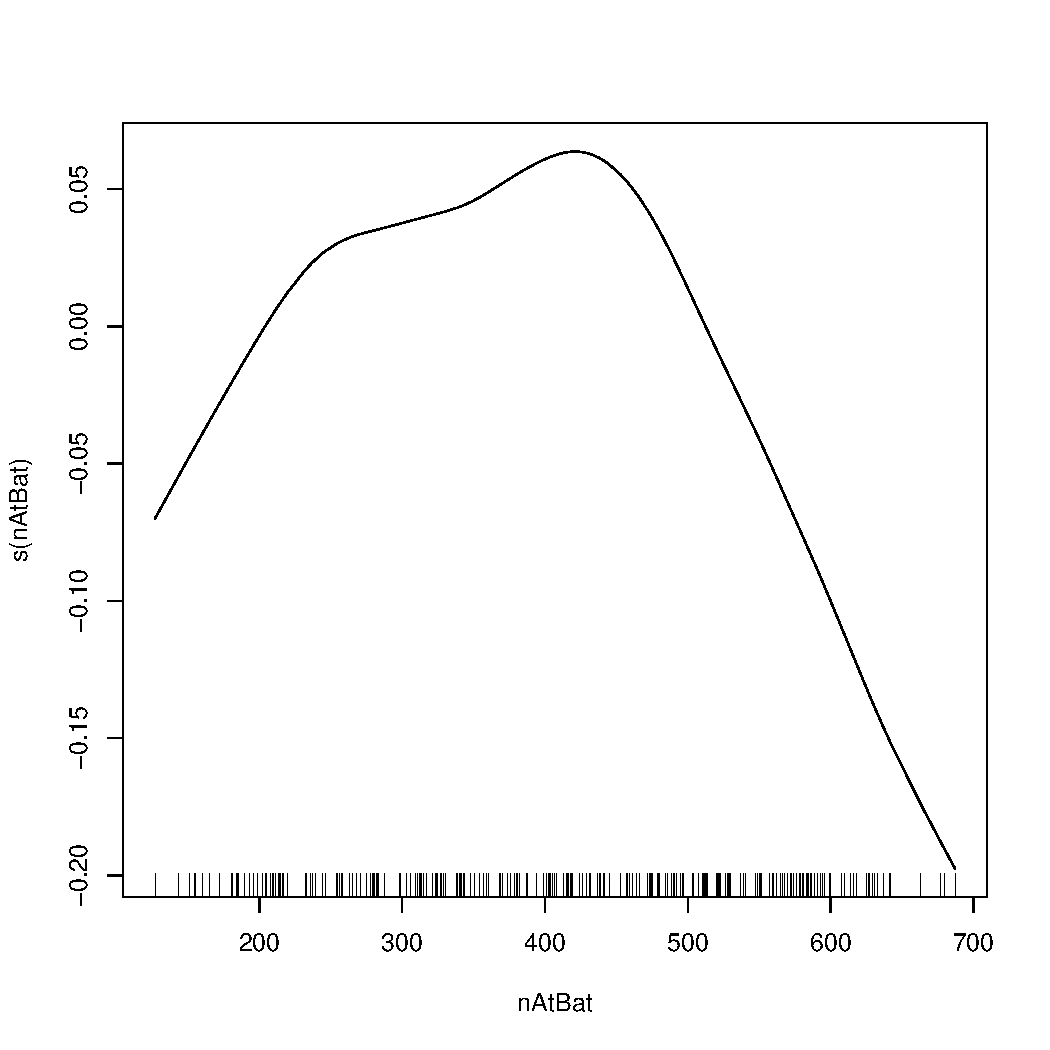
\includegraphics[width=0.50\textwidth]{figure/unnamed-chunk-3-1} 
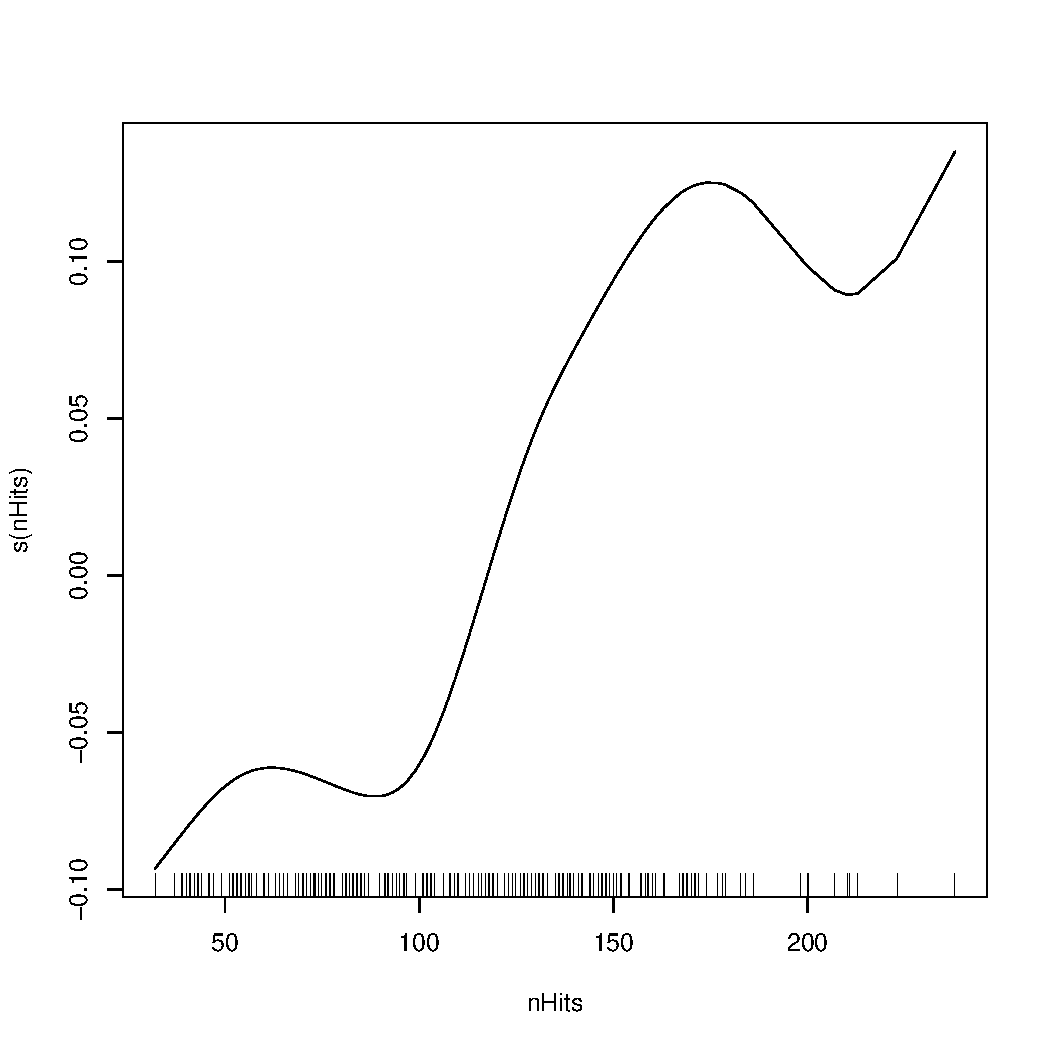
\includegraphics[width=0.50\textwidth]{figure/unnamed-chunk-3-2} 
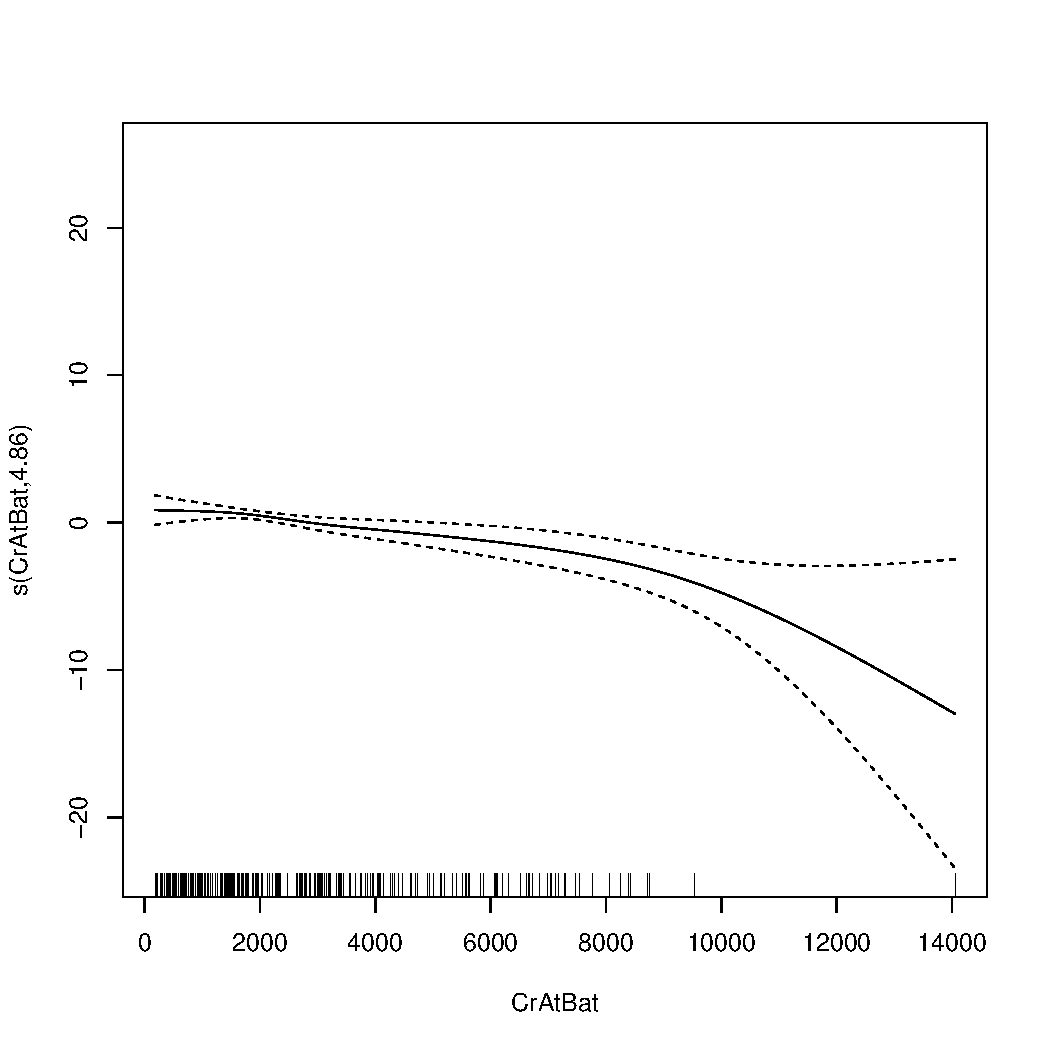
\includegraphics[width=0.50\textwidth]{figure/unnamed-chunk-3-3} 
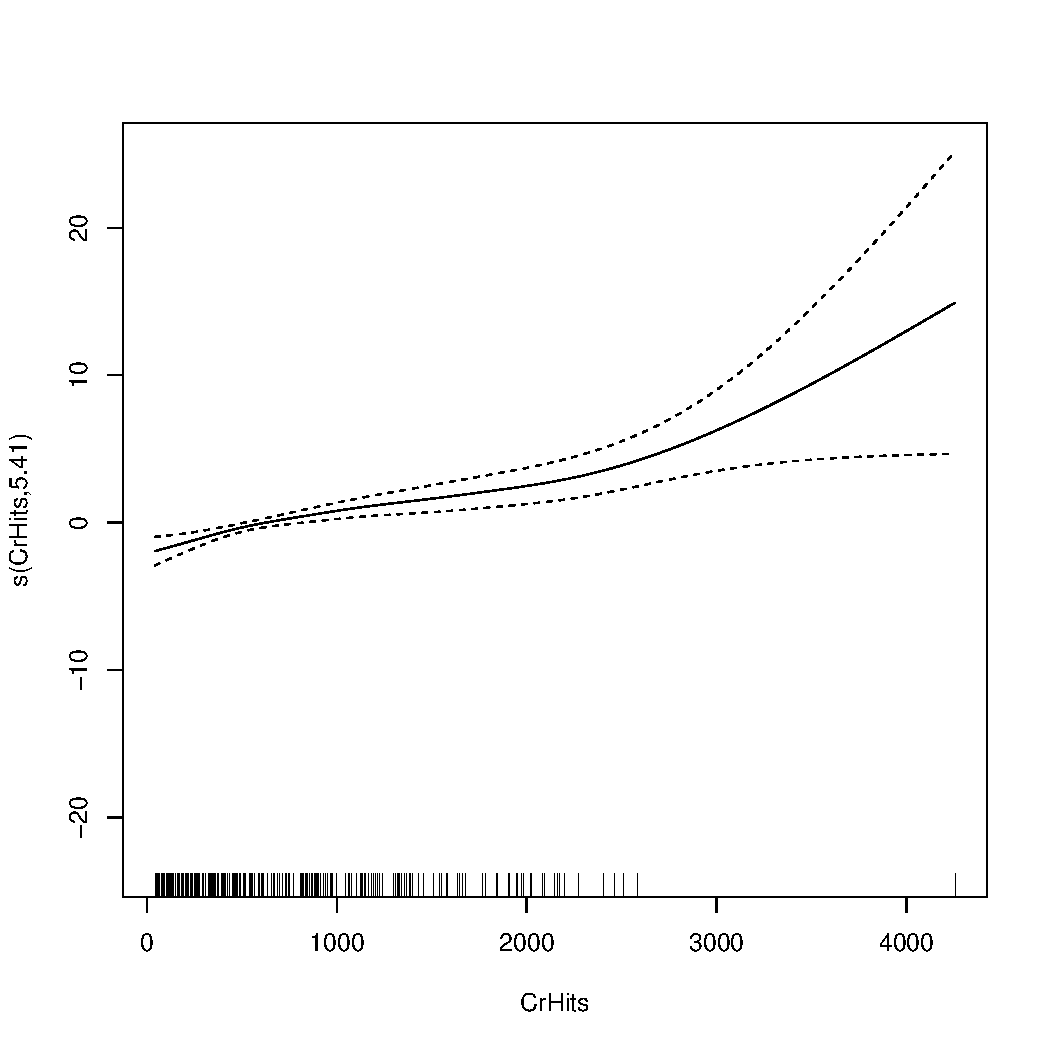
\includegraphics[width=0.50\textwidth]{figure/unnamed-chunk-3-4} 
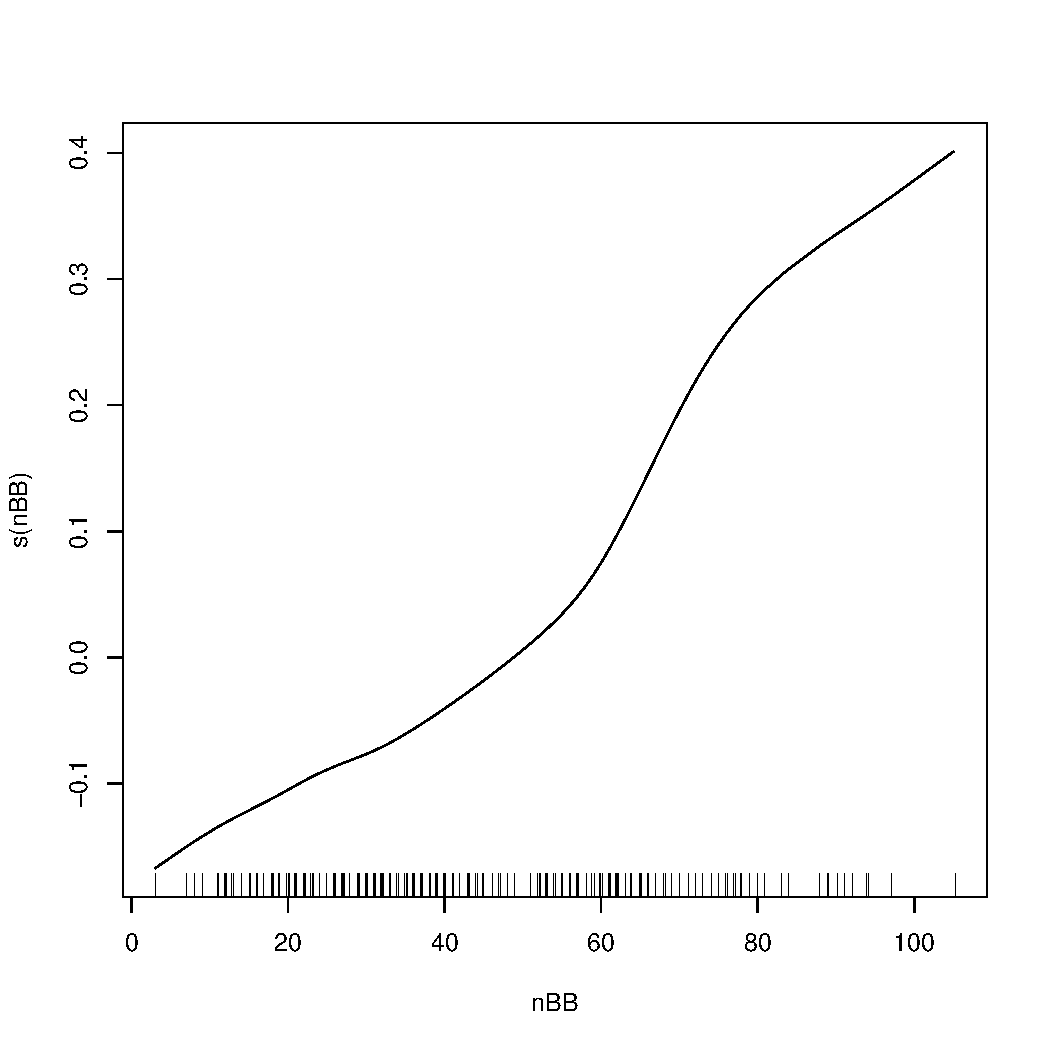
\includegraphics[width=0.50\textwidth]{figure/unnamed-chunk-3-5} 
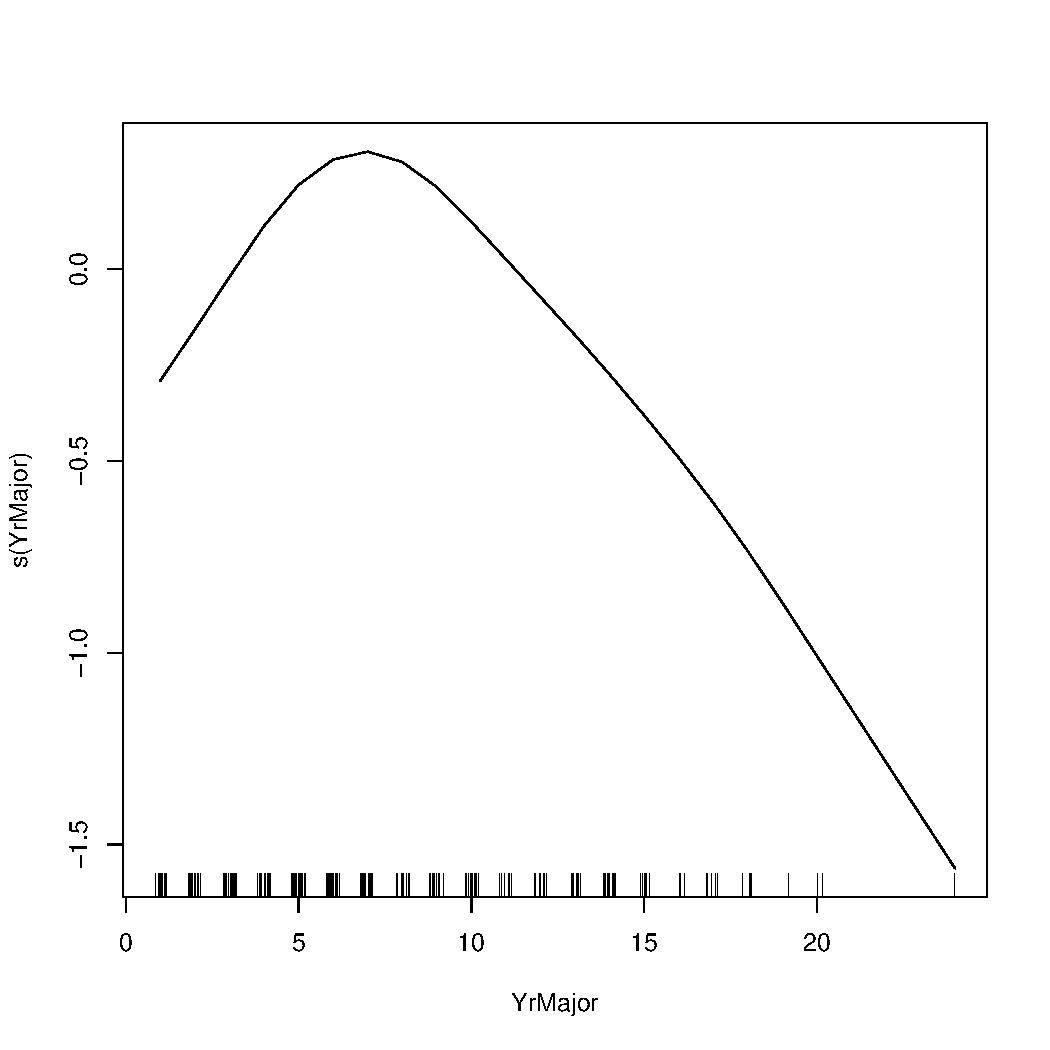
\includegraphics[width=0.50\textwidth]{figure/unnamed-chunk-3-6} 
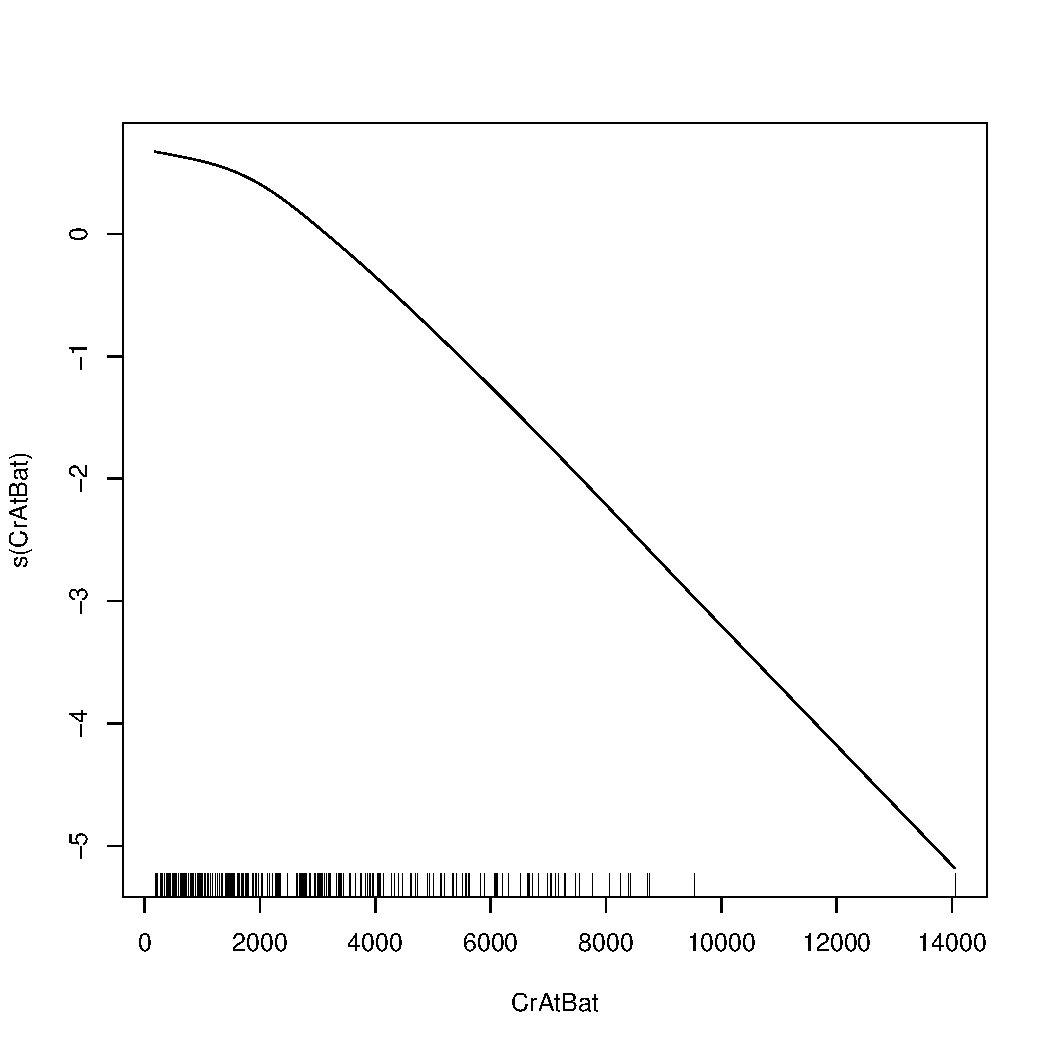
\includegraphics[width=0.50\textwidth]{figure/unnamed-chunk-3-7} 
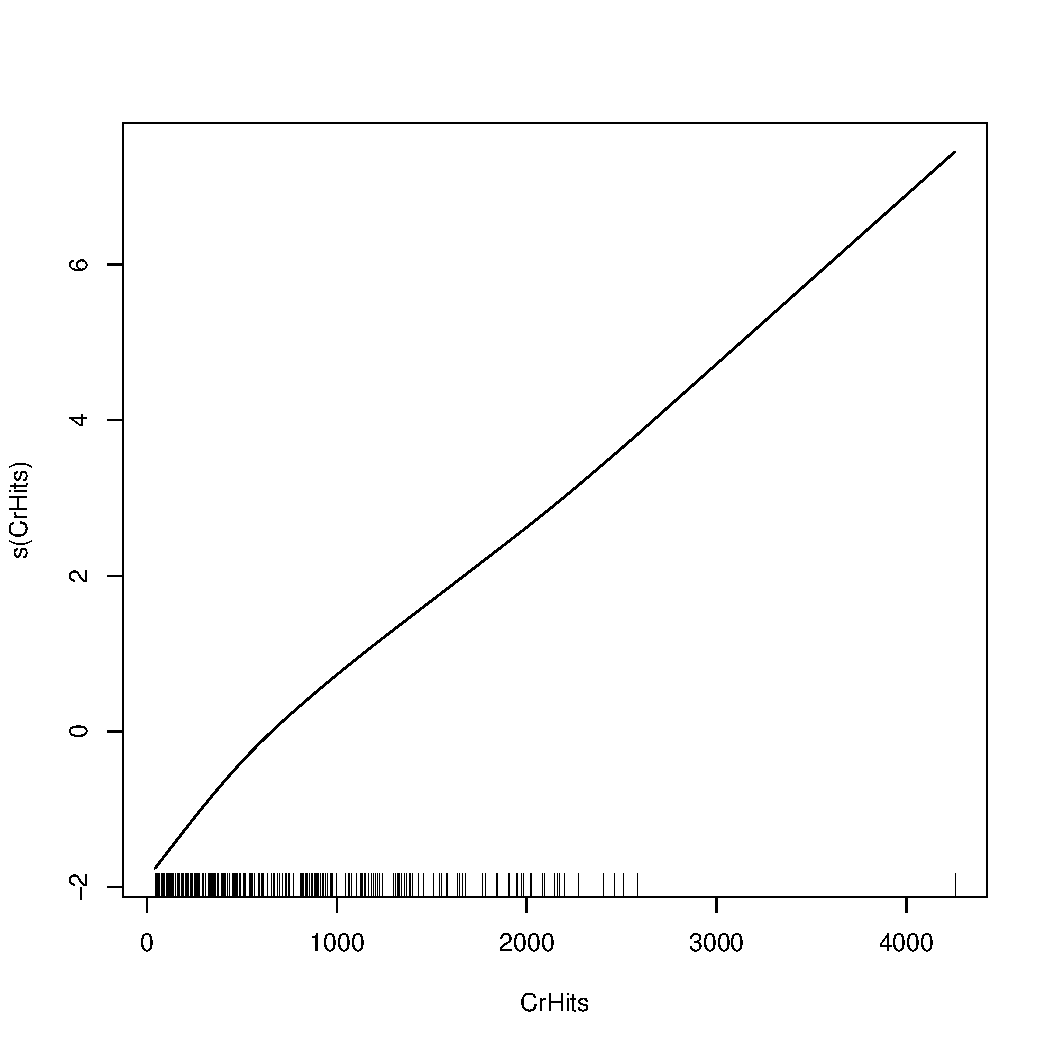
\includegraphics[width=0.50\textwidth]{figure/unnamed-chunk-3-8} 
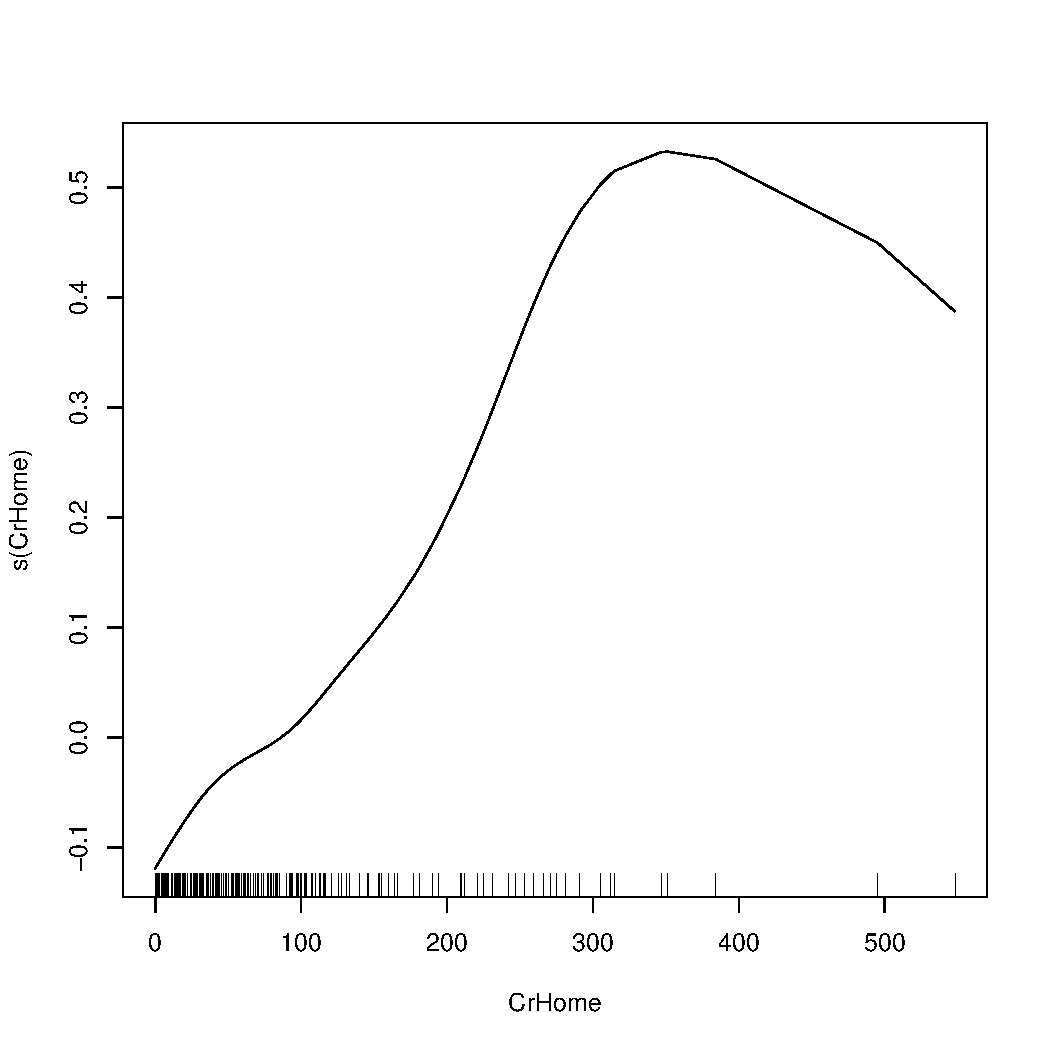
\includegraphics[width=0.50\textwidth]{figure/unnamed-chunk-3-9} 

\end{knitrout}

For simplicity, if we fit a GAM with just CrAtBat and nBB (like we did in the LOESS example), then we get the following surface plot:

\begin{figure}[H]
	\centering
	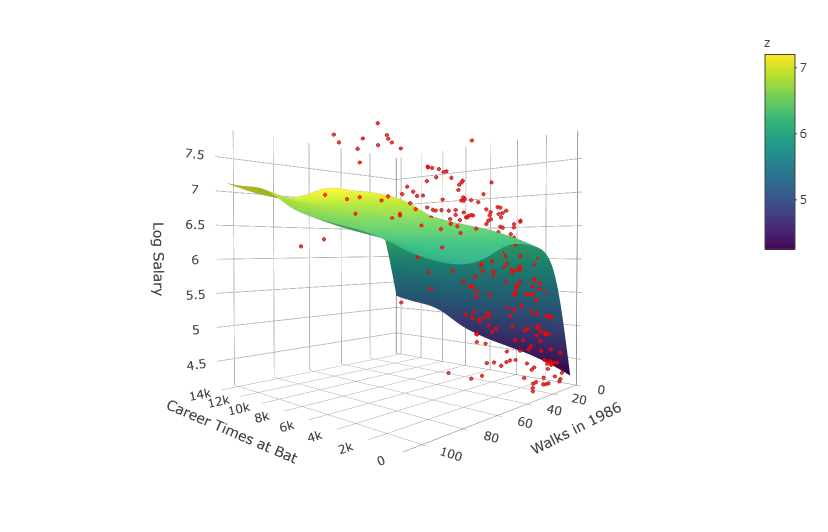
\includegraphics[width=0.6\textwidth]{gam_baseball_demo.png}
	\label{fig:myfig}
\end{figure}

This plot is comparable to the plot from the LOESS example in 4.3.1.

\bigskip
\hrule
\bigskip

\section*{Example 2: Diabetes Dataset}

The Pima Indians Diabetes dataset is a dataset from the National Institute of Diabetes and Digestive and Kidney Diseases. Our goal here is to predict whether or not a patient has diabetes. In this dataset, all patients are females that are at least 21 and are of Pima Indian heritage.

Let's split our data into a training and testing dataset and see how well we do on the testing dataset by training on the training dataset.

\begin{knitrout}
\definecolor{shadecolor}{rgb}{0.969, 0.969, 0.969}\color{fgcolor}\begin{kframe}
\begin{alltt}
\hlkwd{data}\hlstd{(}\hlstr{"diabetes"}\hlstd{)}
\hlkwd{head}\hlstd{(diabetes)}
\end{alltt}
\begin{verbatim}
##   Pregnancies Glucose BloodPressure SkinThickness Insulin  BMI
## 1           6     148            72            35       0 33.6
## 2           1      85            66            29       0 26.6
## 3           8     183            64             0       0 23.3
## 4           1      89            66            23      94 28.1
## 5           0     137            40            35     168 43.1
## 6           5     116            74             0       0 25.6
##   DiabetesPedigreeFunction Age Outcome
## 1                    0.627  50       1
## 2                    0.351  31       0
## 3                    0.672  32       1
## 4                    0.167  21       0
## 5                    2.288  33       1
## 6                    0.201  30       0
\end{verbatim}
\begin{alltt}
\hlcom{# How many observations are there?}
\hlkwd{nrow}\hlstd{(diabetes)}
\end{alltt}
\begin{verbatim}
## [1] 768
\end{verbatim}
\begin{alltt}
\hlcom{# Create a training and testing split with 80% training data}
\hlstd{train_index} \hlkwb{<-} \hlkwd{sample}\hlstd{(}\hlnum{1}\hlopt{:}\hlkwd{nrow}\hlstd{(diabetes),} \hlkwc{size} \hlstd{=} \hlnum{0.80}\hlopt{*}\hlkwd{nrow}\hlstd{(diabetes))}
\hlstd{diabetes_train} \hlkwb{<-} \hlstd{diabetes[train_index, ]}
\hlstd{diabetes_test} \hlkwb{<-} \hlstd{diabetes[}\hlopt{-}\hlstd{train_index, ]}

\hlstd{diabetes_gam} \hlkwb{<-} \hlstd{gam}\hlopt{::}\hlkwd{gam}\hlstd{(Outcome} \hlopt{~} \hlkwd{s}\hlstd{(Pregnancies)} \hlopt{+} \hlkwd{s}\hlstd{(Glucose)} \hlopt{+} \hlkwd{s}\hlstd{(BloodPressure)} \hlopt{+}
                           \hlkwd{s}\hlstd{(SkinThickness)} \hlopt{+} \hlkwd{s}\hlstd{(Insulin)} \hlopt{+} \hlkwd{s}\hlstd{(BMI)} \hlopt{+}
                           \hlkwd{s}\hlstd{(DiabetesPedigreeFunction)} \hlopt{+} \hlkwd{s}\hlstd{(Age),} \hlkwc{family} \hlstd{=} \hlstr{"binomial"}\hlstd{,}
                         \hlkwc{data} \hlstd{= diabetes_train)}
\end{alltt}
\end{kframe}
\end{knitrout}

Now let's see how accurate we are on the testing dataset:

\begin{knitrout}
\definecolor{shadecolor}{rgb}{0.969, 0.969, 0.969}\color{fgcolor}\begin{kframe}
\begin{alltt}
\hlcom{# Here are the predicted class probabilities}
\hlstd{test_class_prob} \hlkwb{<-} \hlkwd{predict}\hlstd{(diabetes_gam, diabetes_test,} \hlkwc{type} \hlstd{=} \hlstr{"response"}\hlstd{)}

\hlcom{# If the probability is higher than 50% of having diabetes, mark it as a 1.}
\hlstd{pred_class} \hlkwb{<-} \hlkwd{rep}\hlstd{(}\hlnum{0}\hlstd{,} \hlkwd{nrow}\hlstd{(diabetes_test))}
\hlstd{pred_class[test_class_prob} \hlopt{>} \hlnum{0.50}\hlstd{]} \hlkwb{<-} \hlnum{1}

\hlcom{# Now that we have our predicted class, let's get some statistics on our accuracy.}
\hlstd{total_test} \hlkwb{<-} \hlkwd{nrow}\hlstd{(diabetes_test)}
\hlstd{total_correct} \hlkwb{<-} \hlkwd{sum}\hlstd{(pred_class} \hlopt{==} \hlstd{diabetes_test}\hlopt{$}\hlstd{Outcome)}

\hlcom{# Error rate}
\hlstd{(total_test} \hlopt{-} \hlstd{total_correct)} \hlopt{/} \hlstd{total_test}
\end{alltt}
\begin{verbatim}
## [1] 0.3116883
\end{verbatim}
\begin{alltt}
\hlcom{# Successful prediction rate}
\hlstd{total_correct} \hlopt{/} \hlstd{total_test}
\end{alltt}
\begin{verbatim}
## [1] 0.6883117
\end{verbatim}
\end{kframe}
\end{knitrout}

\end{document}
